%%%%%%%%%%%%%%%%%%%%%%%%%%%%%%%%%%%%%%%%%
% Jacobs Landscape Poster
% LaTeX Template
% Version 1.0 (29/03/13)
%
% Created by:
% Computational Physics and Biophysics Group, Jacobs University
% https://teamwork.jacobs-university.de:8443/confluence/display/CoPandBiG/LaTeX+Poster
% 
% Further modified by:
% Nathaniel Johnston (nathaniel@njohnston.ca)
%
% This template has been downloaded from:
% http://www.LaTeXTemplates.com
%
% License:
% CC BY-NC-SA 3.0 (http://creativecommons.org/licenses/by-nc-sa/3.0/)
%
%%%%%%%%%%%%%%%%%%%%%%%%%%%%%%%%%%%%%%%%%

%----------------------------------------------------------------------------------------
%	PACKAGES AND OTHER DOCUMENT CONFIGURATIONS
%----------------------------------------------------------------------------------------

\documentclass[final]{beamer}

\usepackage[scale=1.24]{beamerposter} % Use the beamerposter package for laying out the poster

\usetheme{confposter} % Use the confposter theme supplied with this template

\setbeamercolor{block title}{fg=jblue,bg=white} % Colors of the block titles
\setbeamercolor{block body}{fg=black,bg=white} % Colors of the body of blocks
\setbeamercolor{block alerted title}{fg=white,bg=YellowOrange} % Colors of the highlighted block titles
\setbeamercolor{block alerted body}{fg=black,bg=YellowOrange!10} % Colors of the body of highlighted blocks
% Many more colors are available for use in beamerthemeconfposter.sty

%-----------------------------------------------------------
% Define the column widths and overall poster size
% To set effective sepwid, onecolwid and twocolwid values, first choose how many columns you want and how much separation you want between columns
% In this template, the separation width chosen is 0.024 of the paper width and a 4-column layout
% onecolwid should therefore be (1-(# of columns+1)*sepwid)/# of columns e.g. (1-(4+1)*0.024)/4 = 0.22
% Set twocolwid to be (2*onecolwid)+sepwid = 0.464
% Set threecolwid to be (3*onecolwid)+2*sepwid = 0.708

\newlength{\sepwid}
\newlength{\onecolwid}
\newlength{\twocolwid}
\newlength{\threecolwid}
\setlength{\paperwidth}{48in} % A0 width: 46.8in
\setlength{\paperheight}{36in} % A0 height: 33.1in
\setlength{\sepwid}{0.024\paperwidth} % Separation width (white space) between columns
\setlength{\onecolwid}{0.22\paperwidth} % Width of one column
\setlength{\twocolwid}{0.464\paperwidth} % Width of two columns
\setlength{\threecolwid}{0.708\paperwidth} % Width of three columns
\setlength{\topmargin}{-0.5in} % Reduce the top margin size
%-----------------------------------------------------------

\usepackage{graphicx}  % Required for including images

\usepackage{booktabs} % Top and bottom rules for tables

%----------------------------------------------------------------------------------------
%	TITLE SECTION 
%----------------------------------------------------------------------------------------

\title{Digital Participation: New Awareness of Oracy}
%\title{Master's Dissertation Module: Presentation as Formative Assessment} % Poster title

\author{Maria Kunilovskaya (1821716)} % Author(s)

\institute{7ED050 Contemporary Challenges and Opportunities in Higher Education} % Institution(s)

%----------------------------------------------------------------------------------------

\begin{document}

\addtobeamertemplate{block end}{}{\vspace*{2ex}} % White space under blocks
\addtobeamertemplate{block alerted end}{}{\vspace*{2ex}} % White space under highlighted (alert) blocks

\setlength{\belowcaptionskip}{2ex} % White space under figures
\setlength\belowdisplayshortskip{2ex} % White space under equations

\begin{frame}[t] % The whole poster is enclosed in one beamer frame
\begin{picture}(0,0)
\put(100,150){
\includegraphics[width=0.17\linewidth]{pics/work-from-home.png}}
\end{picture}
\begin{columns}[t] % The whole poster consists of three major columns, the second of which is split into two columns twice - the [t] option aligns each column's content to the top

\begin{column}{\sepwid}\end{column} % Empty spacer column

\begin{column}{\onecolwid} % The first column

%----------------------------------------------------------------------------------------
%	MOTIVATION and CONTEXT
%----------------------------------------------------------------------------------------
\setbeamercolor{block alerted title}{fg=jblue,bg=YellowOrange} % Change the alert block title colors
\begin{alertblock}{Motivation and Aims}

\textit{Online learning (and a digitalised world of work) calls for skills in digital communication and puts new pressures, inc. wrt quality of shared content}\\
\medskip
\textbf{\textcolor{dgreen}{Aims}}:
\begin{itemize}
\item explore oracy in the HE context
\item trace its role to enhance learning experience
\item propose a way to bring academic oracy to MA
\end{itemize}
\textbf{\textcolor{dgreen}{Context: a competitive European Masters, all students are international}}

\end{alertblock}

%----------------------------------------------------------------------------------------
%	DEFINITION and RELATED
%----------------------------------------------------------------------------------------

\begin{block}{Oracy in a Digital World}

\begin{itemize}
\item Oracy is the mastery of spoken language (speaking and listening).
\item genres: taking part in a debate, presenting a prepared monologue and group work
\item Digital oracy is a hybrid communication skill: digital design, recording and editing video, communicating data.
\item ``one of the most desired graduate employability skills'' (Jackson, 2014)
\item Communication is listed among most sought-after 14 new foundation skills in 2019 (It appears in 40\% of job posting in future-oriented smart cities).
\end{itemize}
\begin{figure}
	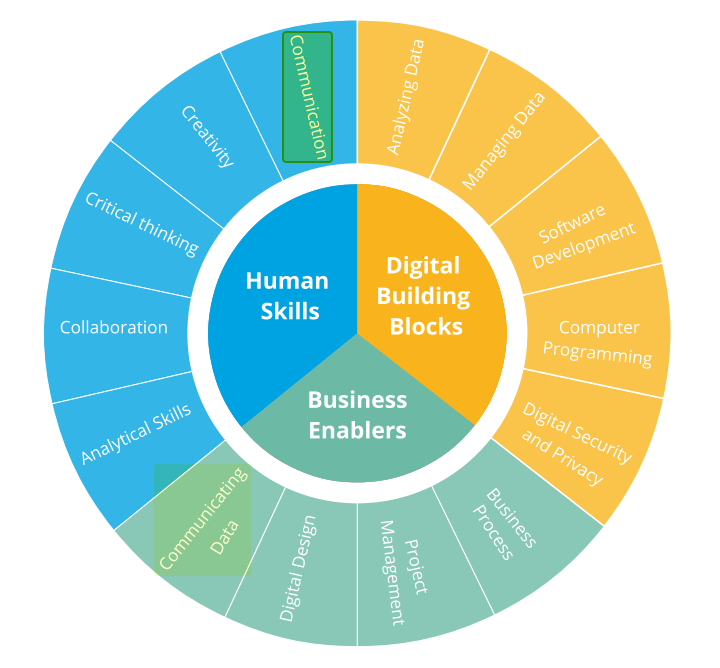
\includegraphics[width=0.7\linewidth]{pics/new_skills.png}
	\caption{New Foundational Skills}
%	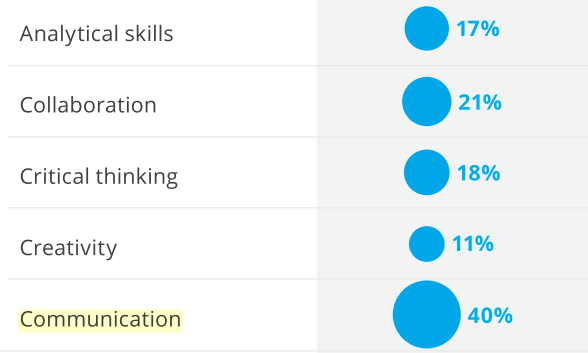
\includegraphics[width=0.7\linewidth]{pics/JobOfferings_w_HumanSkillsRequired_SmartCities.png}
%	\caption{How Often Human Skills are mentioned in Job Postings in Smart Cities}
\end{figure}

\end{block}


\end{column} % End of the first column

\begin{column}{\sepwid}\end{column} % Empty spacer column

\begin{column}{\twocolwid} % Begin a column which is two columns wide (column 2)

\begin{columns}[t,totalwidth=\twocolwid] % Split up the two columns wide column

\begin{column}{\onecolwid}\vspace{-.6in} % The first column within column 2 (column 2.1)

%----------------------------------------------------------------------------------------
%	REQUIREMENTS and EVIDENCE
%----------------------------------------------------------------------------------------

\begin{block}{Context Analysis}

\textbf{\textcolor{dgreen}{Requirements}}:
\begin{itemize}
\item UK Quality Code: "holders of the qualification will be able .. to communicate [their findings] accurately and reliably" "in a variety of forms to specialist and non-specialist audiences."
\item digital capabilities and EdTech are focused in UK strategy in education 2019 (9)
\end{itemize}

\textbf{\textcolor{dgreen}{Gaping Issues}}:
\begin{itemize}
\item oracy was dropped from GSCE in 2014 allegedly for lack of robust marking
\item few opportunities to practice
\item an important medium for participation, but not an explicit product
\item disruptive digital environments are here to stay and favour written interaction

\end{itemize}

\end{block}

%----------------------------------------------------------------------------------------

\end{column} % End of column 2.1

\begin{column}{\onecolwid}\vspace{-.6in} % The second column within column 2 (column 2.2)

%----------------------------------------------------------------------------------------
%	CHANGES needed to achieve the result
%----------------------------------------------------------------------------------------

\begin{block}{Proposed Embedding to MA}

\begin{itemize}
\item include it as part of Dissertation module each year (written::spoken 70/30\%)
\item set up a mock conference (a real audience and purpose for the speech and Q\&A) 
\item require a video-recording of the talk
\item provide conditions for students' self and peer assessment based on analytic formative judgments (use a assessment sheet leading to awards nominations)
\end{itemize}
\textbf{\textcolor{dgreen}{Presentation Rubric}}
\begin{itemize}
	\item components of the rhetoric framework as criteria (Mercer 2017)
	\begin{itemize}
		\item physical (voice, body language)
		\item linguistic (vocabulary, rhetorical techniques)
		\item cognitive (choice of content, reasoning, time-management)
		\item social (audience awareness, liveliness and flair)
	\end{itemize}
	\item sanity of the visual support (slides), digital design
\end{itemize}

\end{block}


\end{column} % End of column 2.2

\end{columns} % End of the split of column 2 - any content after this will now take up 2 columns width


\begin{columns}[t,totalwidth=\twocolwid] % Split up the two columns wide column again

\begin{column}{\onecolwid} % The first column within column 2 (column 2.1)

\begin{block}{New Opportunities and Evidence}
\textbf{\textcolor{dgreen}{Advantages}}
\begin{itemize}
	\item new technology, unprecedented participation: more students are noticed to speak up from the comforts of their homes and no immediate face threats
	\item English as a Lingua Franca (ELF): re-think student support for oracy based on evidence of the same skills in the core of academic oracy
	\item UoW has comparatively developed digital support, inc. Portfolium (PebblePad)
\end{itemize}
\textbf{\textcolor{dgreen}{Empirical evidence for oracy in HE)}}:
\begin{itemize}
\item improved confidence and perceptions of self-efficacy (Campbell, 2020)
\item promotes participation
\item strong link to cognition (Vass and Littleton, 2010)
\item reinforced learning: videos can be more engaging by involving emotions
\item helps with self-reflection
\end{itemize}



\end{block}

%----------------------------------------------------------------------------------------

\end{column} % End of column 2.1

\begin{column}{\onecolwid} % The second column within column 2 (column 2.2)



\begin{block}{Challenges}

\begin{itemize}
	\item To be heard can be difficult, esp in real time (student/teacher ratio: 20.3).
	\item Students need to allocate extra time and resources to develop oracy.
	\item Learning to use a video-editing tool is another challenge (and making the right choice of (free?) software) (ex. kde vs Adobe Premiere).
	\item Students require more experience and training to support academic video production (see a framework proposed in Campbell, 2018)
	\item Credits for the Dissertation module need to be redistributed to incorporate the new assignments involving oracy components
\end{itemize}

\begin{figure}
	
\includegraphics[width=0.2\linewidth]{pics/video.png}
	\caption{Lights, camera, action!}
\end{figure}

\end{block}

%----------------------------------------------------------------------------------------

\end{column} % End of column 2.2

\end{columns} % End of the split of column 2

\end{column} % End of the second column

\begin{column}{\sepwid}\end{column} % Empty spacer column

\begin{column}{\onecolwid} % The third column

\begin{figure}

\includegraphics[width=0.3\linewidth]{pics/oracy.jpeg}
\end{figure}


%----------------------------------------------------------------------------------------
%	CONCLUSION
%----------------------------------------------------------------------------------------

\setbeamercolor{block alerted title}{fg=jblue,bg=YellowOrange} % Change the alert block title colors
\setbeamercolor{block alerted body}{fg=black,bg=YellowOrange!5} % Change the alert block body colors

\begin{alertblock}{Conclusion}

\begin{itemize}
\item The recent shift to greater digitalisation of HE is a transformative opportunity for oracy.
\item Video oracy deserves more attention (esp. with the advent of distance and digital learning), as it is part of digital fluency.
\item It is important to recognise and foster oracy by course designs: create opportunities and scaffold student video generation.
\item Embedding oracy skills will provide all students with equitable opportunities for participation.
\item Student-created video is an active personalized learning activity in an online environment (Campbell, 2020)
\end{itemize}


\end{alertblock}

%----------------------------------------------------------------------------------------
%	REFERENCES
%----------------------------------------------------------------------------------------

\begin{block}{References}
\tiny	
	\begin{enumerate}
		\item Mercer, N., Warwick, P. and Ahmed, A. (2017) An oracy assessment toolkit: Linking research and development in the assessment of students’ spoken language skills at age 11-12, Learning and Instruction, 48, pp. 51–60.
		\item Heron, M. (2019) Making the case for oracy skills in higher education: practices and opportunities, Journal of University Teaching \& Learning Practice, 16(2).
		\item The Frameworks for Higher Education Qualifications of UK Degree-Awarding Bodies (2014), (October).
		\item Vass, E., \& Littleton, K. (2010). Peer collaboration and learning in the classroom. In K. Littleton, C. Wood, \& J. K. Staarman (Eds.), International handbook of psychology in education (pp. 105-136). Leeds: Emerald.
		\item Heron, M. (2019) Making the case for oracy skills in higher education: practices and opportunities, Journal of University Teaching \& Learning Practice, 16(2).
		\item Jackson, D. (2014) Business graduate performance in oral communication skills and strategies for improvement, International Journal of Management Education, vol. 12, no. 1, pp. 22- 34.
		\item University of Wolverhampton TEF3 Provider Submission (2019).
		\item Campbell, Laurie O., Heller, Samantha \& Pulse, Lindsay (2020) Student-created video: an active learning approach in online environments, Interactive Learning Environments
		\item Realising the potential of technology in education: A strategy for education providers and the technology industry (2019)
		\item Campbell, L. O. and Cox, T. D. (2018) Digital Video as a Personalized Learning Assignment: A Qualitative Study of Student Authored Video Using the ICSDR Model, Journal of the Scholarship of Teaching and Learning.
		\item The New Foundational Skills of the Digital Economy. Developing the Professionals of the Future. (2019) Burning Glass / BHEF
		
	\end{enumerate}
	
\end{block}


\includegraphics[width=0.9\linewidth]{pics/wlv-logo-more.jpeg}

%----------------------------------------------------------------------------------------

\end{column} % End of the third column

\end{columns} % End of all the columns in the poster

\end{frame} % End of the enclosing frame

\end{document}
